\documentclass{article}[12pt]
\fontfamily{times}
\usepackage{amsmath, graphicx}
\usepackage[margin=2cm]{geometry}
\usepackage[american]{babel}
\usepackage[style=apa]{biblatex}
\usepackage{booktabs}
\DeclareLanguageMapping{american}{american-apa}
% This is Bob's Bibtex file, won't compile without it
\addbibresource{BibTexDatabase.bib}
\newtheorem{theorem}{Theorem}[section]
\newtheorem{lemma}[theorem]{Lemma}
\newtheorem{proposition}[theorem]{Proposition}
\newtheorem{corollary}[theorem]{Corollary}

\newenvironment{proof}[1][Proof.]{\begin{trivlist}
\item[\hskip \labelsep {\bfseries #1}]}{\end{trivlist}}
\newenvironment{definition}[1][Definition.]{\begin{trivlist}
\item[\hskip \labelsep {\bfseries #1}]}{\end{trivlist}}
\newenvironment{example}[1][Example.]{\begin{trivlist}
\item[\hskip \labelsep {\bfseries #1}]}{\end{trivlist}}
\newenvironment{remark}[1][Remark.]{\begin{trivlist}
\item[\hskip \labelsep {\bfseries #1}]}{\end{trivlist}}

\newcommand{\qed}{\nobreak \ifvmode \relax \else
      \ifdim\lastskip<1.5em \hskip-\lastskip
      \hskip1.5em plus0em minus0.5em \fi \nobreak
      \vrule height0.75em width0.5em depth0.25em\fi}

\begin{document}
%\title{On the Simultaneous Use of Fixed Effects on Cases and Time Points}
\title{Two-Way Fixed Effects: Or How I Learned to Stop Worrying and Just Love Unobserved Heterogeneity}
\date{\today}
\author{Jonathan Kropko\\ University of Virginia \\ jkropko@virginia.edu \and Robert Kubinec \\University of Virginia\\rmk7xy@virginia.edu}
\maketitle
\begin{abstract}
\noindent Time-series cross-sectional (TSCS) data contain a sample of cases observed at repeated time points.  Researchers commonly employ fixed effects (FEs) on the cases to remove cross-sectional unobserved heterogeneity from the model.  Recently, a great deal of applied work includes FEs on cases and on time points in the same model with the intention of accounting for omitted variables in both the cross-sectional and time dimensions.  The properties of the model that includes FEs on both cases and time are not well understood.  We derive the formal two-way FE estimator and show that it does not account for unobserved heterogeneity in either the cross-sectional or the time dimension.  We further demonstrate that the two-way FE model is sensitive to whether the panels are balanced while a model that includes FEs only on cases or only on time points is not.  Using an analysis of the relationship between a country's wealth and level of democracy, we show that the choice of model has a profound influence on the findings.  We recommend that researchers avoid the two-way FE model, and instead use a model with FEs only on cases or only on time points, a choice that depends on the research question. 
\end{abstract}

\newpage

\section{Meta-Analysis}

To examine the prevalence of one and two-way fixed effects models in the political science literature, we collected methodological information on a sample of 363 articles from the \emph{American Political Science Review}, \emph{American Journal of Political Science}, and the \emph{Journal of Politics} for the period 1976 to 2014. The bulk of the articles were collected through JSTOR's Data for Research service, while the most recent years were collected through each journal separately. The search term used to create the dataset was ``fixed effect". Papers that were not one or two-way fixed effects time-series cross section models, such as hierarchical models, random-effects models, and cross-sectional models, were removed.

\begin{figure}
	\centering
	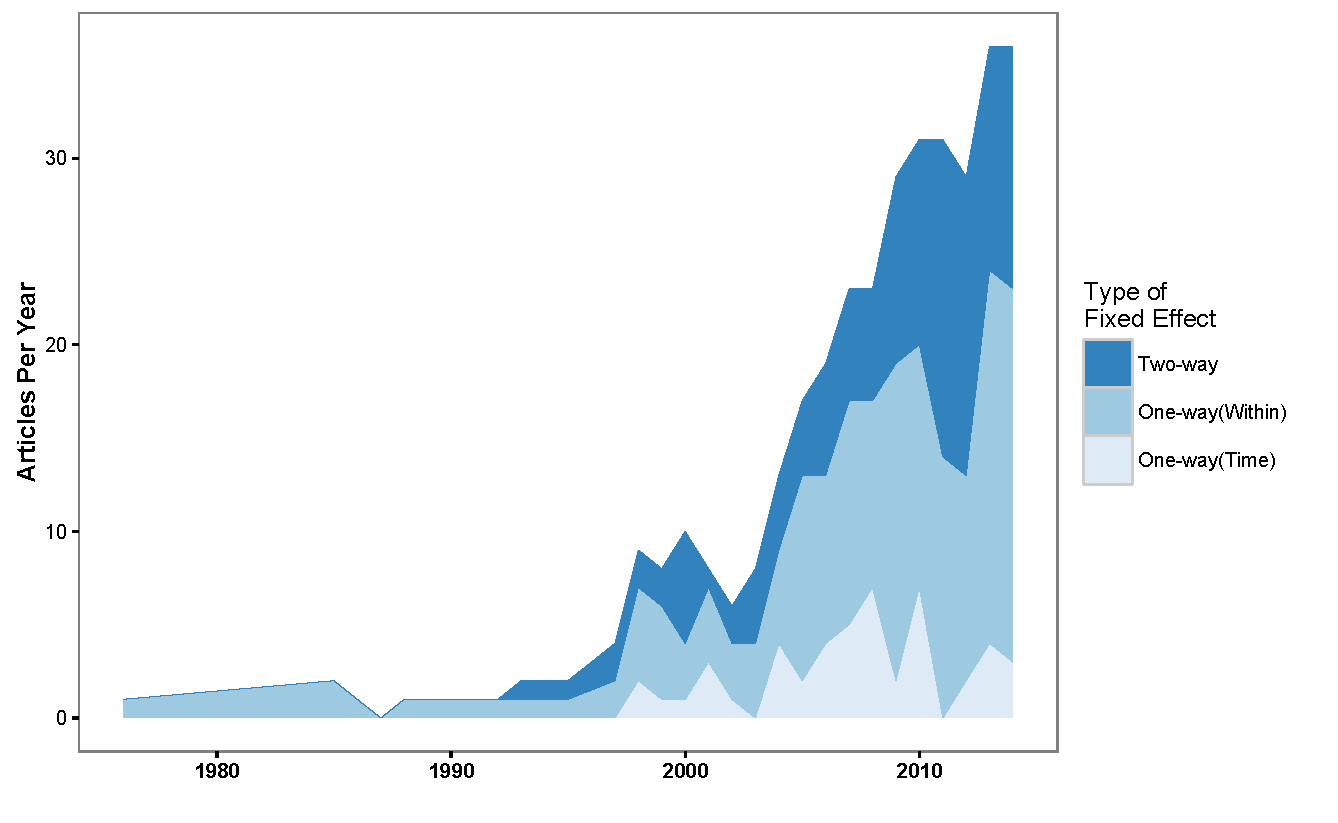
\includegraphics[width=\linewidth]{all_articles}
	\caption{Type of Fixed Effects Employed by Political Science Articles (1976-2014)}\label{allarticles}
\end{figure}

What Figure \ref{allarticles} indicates is that the vast majority of fixed effects models employed in the political science literature are either one-way within models or two-way fixed effects models. In particular, a noticeable trend over the last ten years has been towards greater usage of two-way FEs, although one-way FEs remain the dominant empirical estimation strategy for TSCS data.

What is also evident is that the total number of FE models continue to increase year-on-year. This is likely due to the greater prevalence of TSCS datasets, which we regard as a great asset to the discipline. However, despite these models' greater usage, their interpretation does not appear to have grown more consistent or clear over time. Rather, there are several articles which tend to be frequently cited to justify one empirical strategy or another, with decisions often being made around the limitations of the available data.

Qualitatively, it is apparent that certain papers have guided the bulk of time series cross section in the discipline. \textcite{stimson1985} first presented the ``least-squares with dummy variables" (LSDV) approach, which clarified the nature of fixed effects models although it did not provide specific recommendations as to what kind of one or two-way FX to use. \textcite{beckkatzturner1998} and \textcite{beckkatz1995} advanced the conversation considerably by providing more specific recommendations for how political scientists should run TSCS models depending on the structure of the data, i.e., different ratios of cases versus time points. More recently, alternative to traditional fixed effects models, such as estimation of ``rarely changing variables" \parencite{plumper2007} and difference-in-difference designs \parencite{abadie2005} have diversified fixed effects models to an extent, although the original papers by Beck and Katz and Stimson are still very influential, as can be seen in Figure \ref{stimsonkatz}.

\begin{figure}
	\centering
	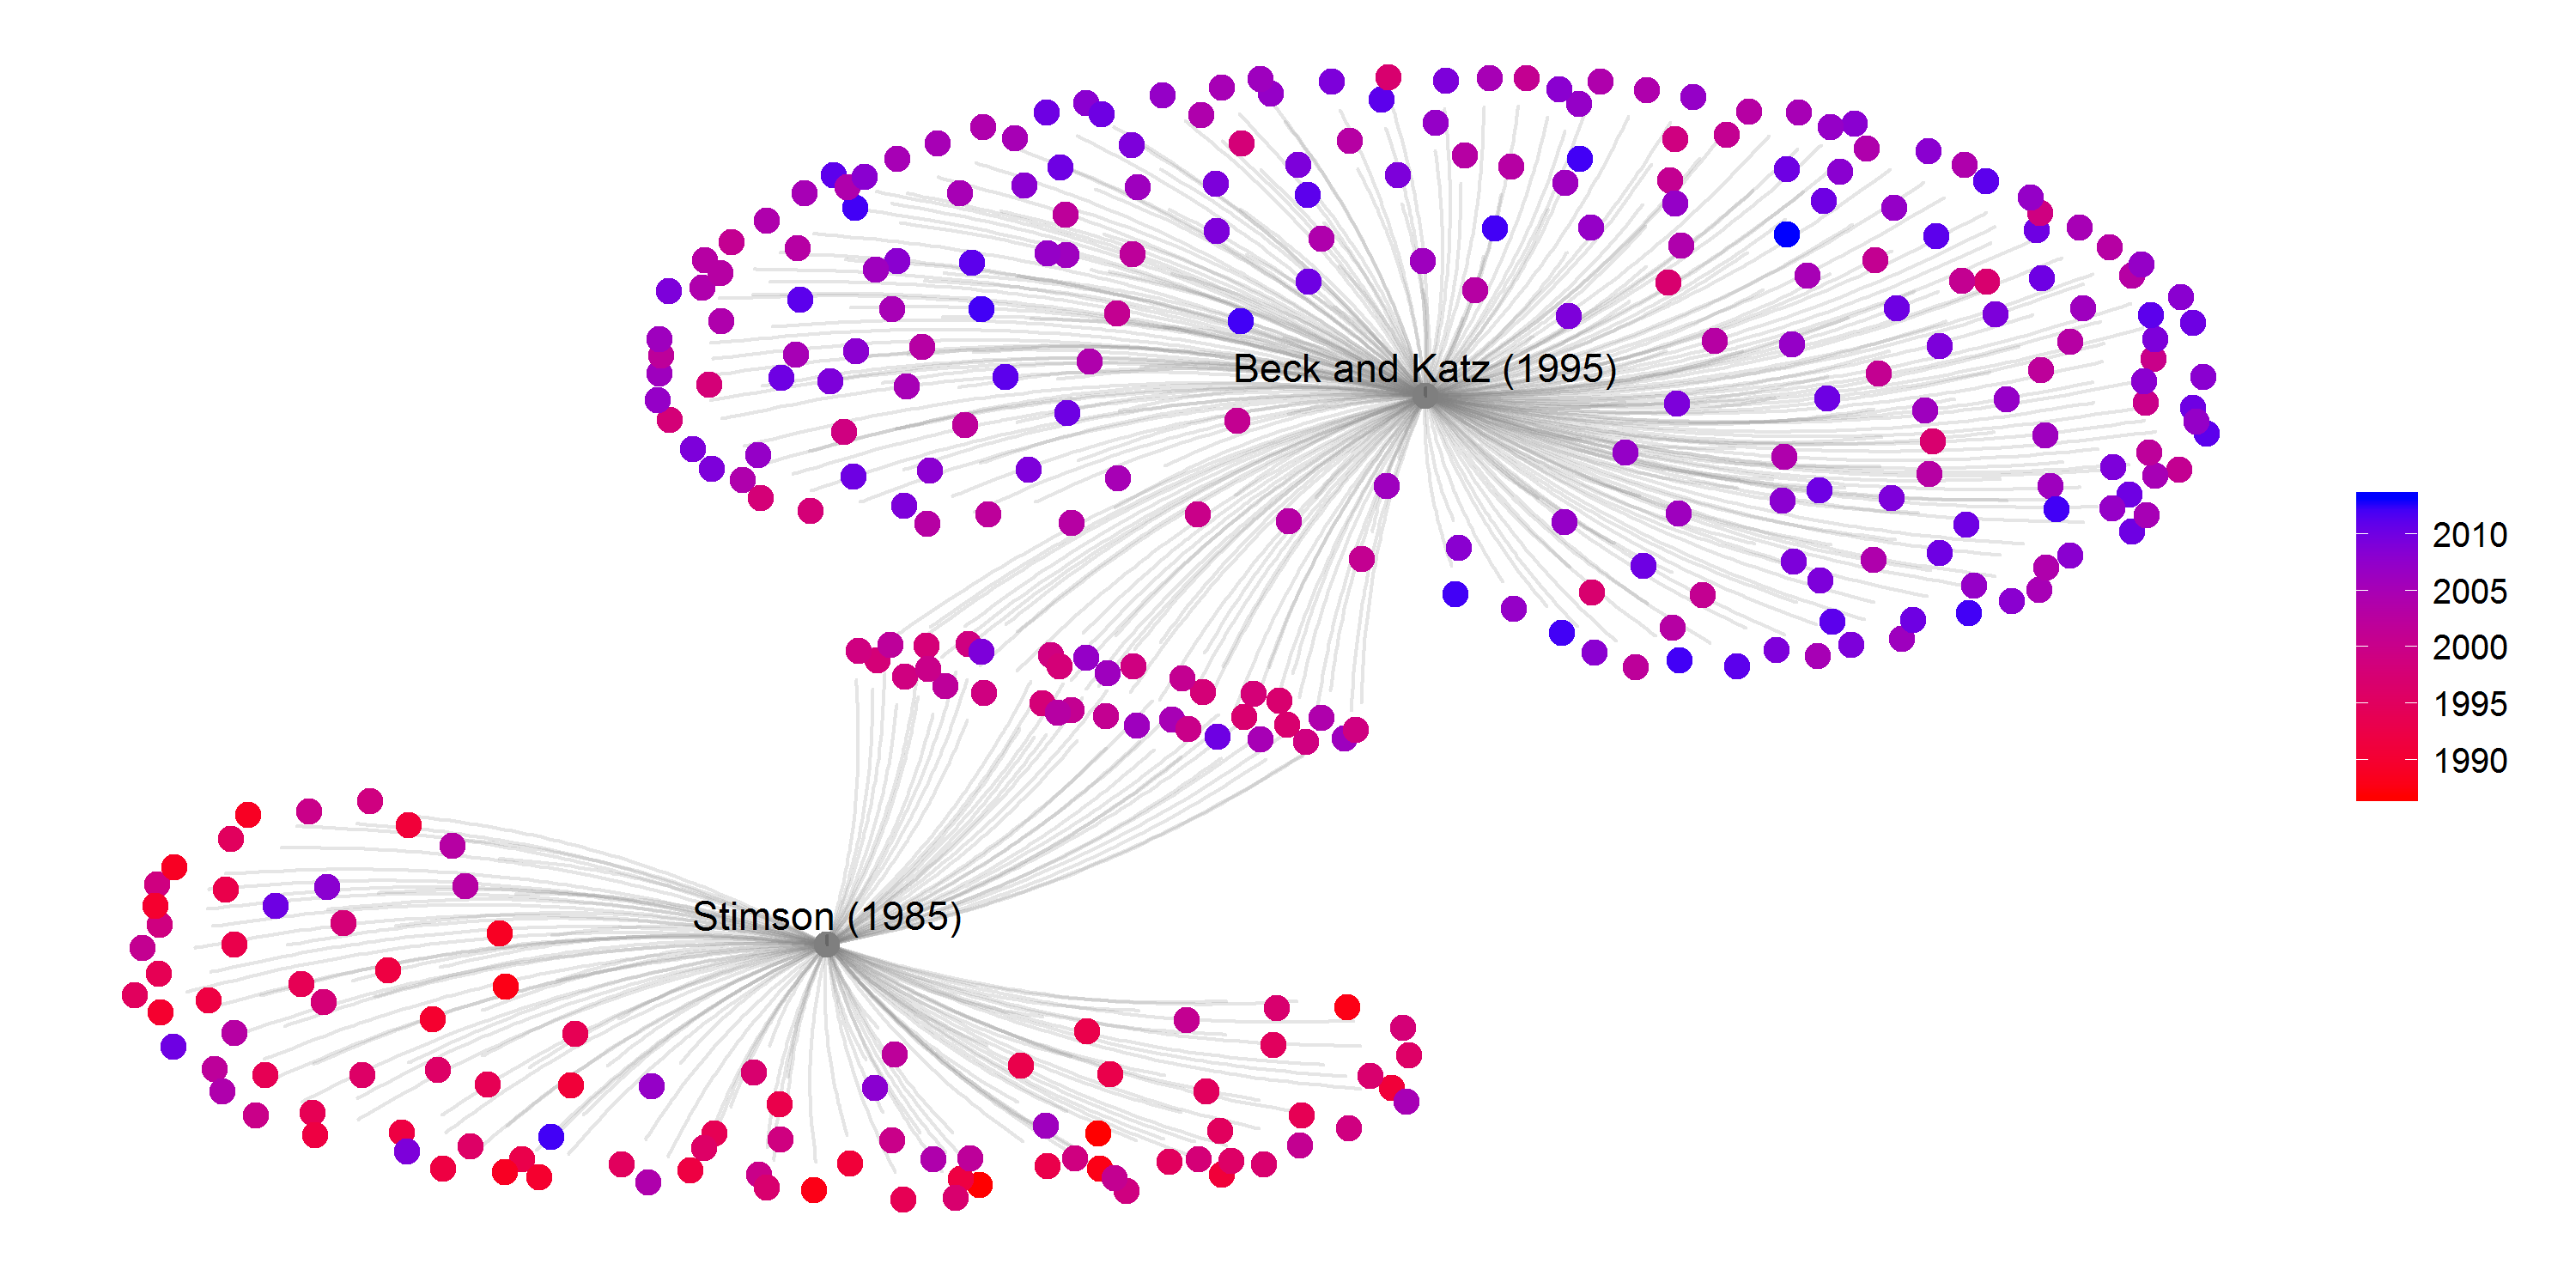
\includegraphics[width=\linewidth]{stimsonkatz}
	\caption{Citations of Beck and Katz (1995) and Stimson (1985) in political science journals in JSTOR}\label{stimsonkatz}
\end{figure}

Yet despite the wide uniformity in methods citations in fixed effects papers, there is also diversity in their interpretation and application. Generally speaking, the econometric notion that fixed effects estimators exist to correct for ``unobserved heterogeneity" [CITE--Wooldridge?] has meant that authors have come to prefer fixed effects for its ability to remove potential confounders. However, there is evident disagreement over what to do when a certain fixed effects model does not fit the data collected, particularly when most of the variables are constant within cases.

Scholars generally use reasoning along the lines of \textcite{donno2013}, who did not use a one-way within FX model because ``fixed effects leads to too many observations dropping from the analysis" (p. 709). The problem, however, is not a lack of statistical power, but rather a mis-application of the within-FX estimator. In \citeauthor{donno2013}'s case, the problem appears to be that she is interested in a variable that does not often change within countries over time, that of the type of electoral system (p. 709). Donno could use a fixed effects model, but as her hypothesis relates more to differences between countries than within countries, a one-way between FX model would probably capture the variation in the dataset more appropriately.

Two-way fixed effects suffer as well from the perception that they are more rigorous than one-way FX models but also require even more data. For example, \textcite{gabel2012} argue that they need both within and between FX because they want to control for ``unobserved national factors" (within FX) and ``temporal shocks" (between FX) (p. 1132). Similarly, \textcite{scheve2012} use two-way FX within their ``difference-in-difference" framework because one-way within FX ``control for time-constant unobserved country-level heterogeneity" while one-way between FX will account for ``common shocks" (p. 82-83).

The use of two-way fixed effects, particularly in terms of the emergent difference-in-difference framework, introduces a new wrinkle in fixed effects estimation. The standard difference-in-difference framework is based on binary time points \parencite{shahidur2010}, but the TSCS application often incorporates many time points. However, authors still refer to the within one-way FX as accounting for ``time-invariant district characteristics" \parencite[484]{anzia2011}. However, these potential confounders are no longer time-invariant with more than two time points \parencite{imai2016}, as potential confounding variables may vary over time both between cases and within cases. 

Given the emphasis on two-way FX and one-way within FX, it is somewhat surprising that one-way FX have been used consistently over the past two decades. However, the identification of fixed effects estimation with either one-way within or two-way FX has meant that one-way between FX models are not always recognized as such, and often their usage depends on traditions within certain streams of scholarship. For example, in the American political science literature on courts, it is common to include fixed effects for the tenure of a court, administration or Congress \parencite{jenkins2012,hall2014,boyd2010,lazarus2009}. This usage highlights the fact that between and within FX are merely two sides of the same coin: they splice up a dataset along two different dimensions, but these dimensions can be relabeled without changing the underlying substance.

\section{Empirical Analysis}

\begin{table}[!htbp] \centering 
	\begin{tabular}{@{\extracolsep{5pt}}lccccc} 

		Variable & \multicolumn{1}{c}{N} & \multicolumn{1}{c}{Mean} & \multicolumn{1}{c}{St. Dev.} & \multicolumn{1}{c}{Min} & \multicolumn{1}{c}{Max} \\ 
		\midrule 
		Log of GDP & 10,445 & 7.812 & 1.023 & 5.315 & 10.667 \\ 
		Electoral Democracy Index & 16,224 & 0.321 & 0.282 & 0.008 & 0.958 \\ 
		\# World Democracies & 10,154 & 30.104 & 7.895 & 13.043 & 48.765 \\ 
		Capital as \% GDP & 5,472 & 0.520 & 0.500 & 0 & 1 \\ 
		Fuel Income Per Capita & 10,211 & 333.186 & 2,251.948 & 0.000 & 81,161.850 \\ 
		Fertility Rate & 10,924 & 4.433 & 2.013 & 0.895 & 9.223 \\ 
		Civil War & 10,089 & 0.066 & 0.247 & 0 & 1 \\ 
	\end{tabular} 
	\caption{Descriptive Statistics} 
	\label{describe} 
\end{table} 

\begin{table}[ht]
\centering

\begin{tabular}{cccccccccc}

 Year & $x_{it}$ & $\bar{x}_i$ & $\bar{x}_b$ & $y_{it}$ & $\bar{y}_i$ &  $(x_{it}  - \bar{x}_t)$ & $(y_{it} - \bar{y}_t)$ & $(x_{it}  - \bar{x}_i)$ & $\frac{(x_{it}  - \bar{x}_i)(y_{it} - \bar{y}_t)}{(x_{it}  - \bar{x}_i)(x_{it} - \bar{x}_t)}$ \\
\midrule
 2001 & 8.02 & 8.31 & 8.12 & 0.40 & 0.51 & -0.10 & -0.10 & -0.30 & -0.15 \\ 2002 & 8.08 & 8.31 & 8.14 & 0.41 & 0.51 & -0.06 & -0.09 & -0.24 & -0.15 \\ 2003 & 8.18 & 8.31 & 8.16 & 0.41 & 0.51 & 0.01 & -0.10 & -0.14 & -0.15 \\ 2004 & 8.30 & 8.31 & 8.20 & 0.37 & 0.51 & 0.09 & -0.14 & -0.01 & -0.15 \\ 2005 & 8.33 & 8.31 & 8.24 & 0.46 & 0.51 & 0.09 & -0.05 & 0.02 & -0.15 \\ 2006 & 8.41 & 8.31 & 8.28 & 0.57 & 0.51 & 0.13 & 0.06 & 0.10 & -0.15 \\ 2007 & 8.49 & 8.31 & 8.33 & 0.62 & 0.51 & 0.17 & 0.11 & 0.18 & -0.15 \\ 2008 & 8.52 & 8.31 & 8.35 & 0.63 & 0.51 & 0.17 & 0.12 & 0.21 & -0.15 \\ 2009 & 8.37 & 8.31 & 8.67 & 0.64 & 0.51 & -0.30 & 0.14 & 0.06 & -0.15 \\ 2010 & 8.42 & 8.31 & 8.71 & 0.56 & 0.51 & -0.29 & 0.05 & 0.11 & -0.15 \\

\end{tabular}
\caption{Two-Way Fixed Effect for Ukraine 2001-2010}\label{Ukraine_table}
\end{table}
	


\section{Proofs}

\textbf{Lemma 1a.}  The following equivalence holds in both balanced and unbalanced panels:
\begin{equation}
\sum_{i=1}^N \sum_{t=1}^{T_i}(x_{it}  - \bar{x}_i)(y_{it}  - \bar{y}_i) = \sum_{i=1}^N \sum_{t=1}^{T_i}(x_{it}  - \bar{x}_i)(y_{it}  - \bar{y})=\sum_{i=1}^N \sum_{t=1}^{T_i} (x_{it}  - \bar{x})(y_{it}  - \bar{y}_i).
\end{equation}
\begin{proof}
We prove the lemma for unbalanced panels, but the lemma also holds for balanced panels since balanced panels are the special case in which $T_i = T_j, \forall i, j \in \{1, \hdots, N\}$. We demonstrate that all three expressions are individually equal to $\sum_{i=1}^N \sum_{t=1}^{T_i}x_{it}y_{it} - \sum_{i=1}^N T_i\bar{x}_i \bar{y}_i$ and are therefore equal to each other:
\begin{align}
\sum_{i=1}^N \sum_{t=1}^{T_i}(x_{it}  - \bar{x}_i)(y_{it}  - \bar{y}_i)  & = \sum_{i=1}^N \sum_{t=1}^{T_i}(x_{it}y_{it} - x_{it}\bar{y}_i  - \bar{x}_iy_{it}  +\bar{x}_i \bar{y}_i) \nonumber\\
& = \sum_{i=1}^N \sum_{t=1}^{T_i}x_{it}y_{it} - \sum_{i=1}^N \sum_{t=1}^{T_i}x_{it}\bar{y}_i  - \sum_{i=1}^N \sum_{t=1}^{T_i}\bar{x}_iy_{it}  + \sum_{i=1}^N \sum_{t=1}^{T_i}\bar{x}_i \bar{y}_i \nonumber\\
& = \sum_{i=1}^N \sum_{t=1}^{T_i}x_{it}y_{it} - \sum_{i=1}^N \bar{y}_i\sum_{t=1}^{T_i}x_{it}  - \sum_{i=1}^N \bar{x}_i\sum_{t=1}^{T_i}y_{it}  + \sum_{i=1}^N T_i\bar{x}_i \bar{y}_i \nonumber\\
& = \sum_{i=1}^N \sum_{t=1}^{T_i}x_{it}y_{it} - \sum_{i=1}^N \bar{y}_i(T_i \bar{x}_i)  - \sum_{i=1}^N \bar{x}_i(T_i\bar{y}_i)  + \sum_{i=1}^N T_i\bar{x}_i \bar{y}_i \nonumber\\
& = \sum_{i=1}^N \sum_{t=1}^{T_i}x_{it}y_{it} - \sum_{i=1}^N T_i\bar{x}_i \bar{y}_i.
\end{align}

\begin{align}
\sum_{i=1}^N \sum_{t=1}^{T_i}(x_{it}  - \bar{x}_i)(y_{it}  - \bar{y})  & = \sum_{i=1}^N \sum_{t=1}^{T_i}(x_{it}y_{it} - x_{it}\bar{y}  - \bar{x}_iy_{it}  +\bar{x}_i \bar{y}) \nonumber\\
& = \sum_{i=1}^N \sum_{t=1}^{T_i}x_{it}y_{it} - \sum_{i=1}^N \sum_{t=1}^{T_i}x_{it}\bar{y}  - \sum_{i=1}^N \sum_{t=1}^{T_i}\bar{x}_iy_{it}  + \sum_{i=1}^N \sum_{t=1}^{T_i}\bar{x}_i \bar{y} \nonumber\\
& = \sum_{i=1}^N \sum_{t=1}^{T_i}x_{it}y_{it} - \bar{y}\sum_{i=1}^N \sum_{t=1}^{T_i}x_{it}  - \sum_{i=1}^N \bar{x}_i\sum_{t=1}^{T_i}y_{it}  + \bar{y}\sum_{i=1}^N T_i\bar{x}_i  \nonumber\\
& = \sum_{i=1}^N \sum_{t=1}^{T_i}x_{it}y_{it} - \bar{y}\sum_{i=1}^N T_i \bar{x}_i  - \sum_{i=1}^N \bar{x}_i(T_i\bar{y}_i)  + \bar{y}\sum_{i=1}^N T_i\bar{x}_i  \nonumber\\
& = \sum_{i=1}^N \sum_{t=1}^{T_i}x_{it}y_{it} - \sum_{i=1}^N T_i\bar{x}_i \bar{y}_i.
\end{align}

\begin{align}
\sum_{i=1}^N \sum_{t=1}^{T_i}(x_{it}  - \bar{x})(y_{it}  - \bar{y}_i)  & = \sum_{i=1}^N \sum_{t=1}^{T_i}(x_{it}y_{it} - x_{it}\bar{y}_i  - \bar{x}y_{it}  +\bar{x} \bar{y}_i) \nonumber\\
& = \sum_{i=1}^N \sum_{t=1}^{T_i}x_{it}y_{it} - \sum_{i=1}^N \sum_{t=1}^{T_i}x_{it}\bar{y}_i  - \sum_{i=1}^N \sum_{t=1}^{T_i}\bar{x}y_{it}  + \sum_{i=1}^N \sum_{t=1}^{T_i}\bar{x} \bar{y}_i \nonumber\\
& = \sum_{i=1}^N \sum_{t=1}^{T_i}x_{it}y_{it} - \sum_{i=1}^N \bar{y}_i\sum_{t=1}^{T_i}x_{it}  - \bar{x}\sum_{i=1}^N \sum_{t=1}^{T_i}y_{it}  + \bar{x}\sum_{i=1}^N T_i \bar{y}_i \nonumber\\
& = \sum_{i=1}^N \sum_{t=1}^{T_i}x_{it}y_{it} - \sum_{i=1}^N \bar{y}_i(T_i \bar{x}_i)  - \bar{x}\sum_{i=1}^N T_i\bar{y}_i + \bar{x}\sum_{i=1}^N T_i \bar{y}_i \nonumber\\
& = \sum_{i=1}^N \sum_{t=1}^{T_i}x_{it}y_{it} - \sum_{i=1}^N T_i\bar{x}_i \bar{y}_i.\qed
\end{align}
\end{proof}
\textbf{Lemma 1b.}  The following equivalence holds in both balanced and unbalanced panels:
\begin{equation}
\sum_{i=1}^N \sum_{t=1}^{T_i}(x_{it}  - \bar{x}_t)(y_{it}  - \bar{y}_t) = \sum_{i=1}^N \sum_{t=1}^{T_i}(x_{it}  - \bar{x}_t)(y_{it}  - \bar{y})=\sum_{i=1}^N \sum_{t=1}^{T_i} (x_{it}  - \bar{x})(y_{it}  - \bar{y}_t).
\end{equation}
\begin{proof}
The proof follows the proof of lemma 1a, substituting $\bar{x}_t$ for $\bar{x}_i$ and $\bar{y}_t$ for $\bar{y}_i$ and rewriting the summation as $\sum_{t=1}^{T}\sum_{i=1}^{N_t}$. \qed
\end{proof}
\textbf{Lemma 2a}. The following equivalence holds in both balanced and unbalanced panels:
\begin{equation}
\sum_{i=1}^N \sum_{t=1}^{T_i}(x_{it}  - \bar{x}_i)^2  = \sum_{i=1}^N \sum_{t=1}^{T_i}(x_{it}  - \bar{x}_i)(x_{it}  - \bar{x}).
\end{equation}
\begin{proof}
We prove the lemma for unbalanced panels, but the lemma also holds for balanced panels since balanced panels are the special case in which $T_i = T_j, \forall i, j \in \{1, \hdots, N\}$. We demonstrate that both expressions are individually equal to $\sum_{i=1}^N \sum_{t=1}^{T_i}x_{it}^2  -  \sum_{i=1}^N T_i\bar{x}_i^2$ and are therefore equal to each other:
\begin{align}
\sum_{i=1}^N \sum_{t=1}^{T_i}(x_{it}  - \bar{x}_i)^2 & = \sum_{i=1}^N \sum_{t=1}^{T_i}(x_{it}^2  - 2x_{it}\bar{x}_i + \bar{x}_i^2)\nonumber\\ 
& = \sum_{i=1}^N \sum_{t=1}^{T_i}x_{it}^2  - 2\sum_{i=1}^N \sum_{t=1}^{T_i}x_{it}\bar{x}_i + \sum_{i=1}^N \sum_{t=1}^{T_i}\bar{x}_i^2\nonumber\\ 
& = \sum_{i=1}^N \sum_{t=1}^{T_i}x_{it}^2  - 2\sum_{i=1}^N \bar{x}_i \sum_{t=1}^{T_i}x_{it}+ \sum_{i=1}^N T_i\bar{x}_i^2\nonumber\\ 
& = \sum_{i=1}^N \sum_{t=1}^{T_i}x_{it}^2  - 2\sum_{i=1}^N T_i\bar{x}_{i}^2+ \sum_{i=1}^N T_i\bar{x}_i^2\nonumber\\ 
& = \sum_{i=1}^N \sum_{t=1}^{T_i}x_{it}^2  -  \sum_{i=1}^N T_i\bar{x}_i^2.
\end{align}

\begin{align}
\sum_{i=1}^N \sum_{t=1}^{T_i}(x_{it}  - \bar{x}_i)(x_{it}  - \bar{x}) & = \sum_{i=1}^N \sum_{t=1}^{T_i}(x_{it}^2  -\bar{x}x_{it} - \bar{x}_ix_{it} + \bar{x}_i\bar{x})\nonumber\\ 
& = \sum_{i=1}^N \sum_{t=1}^{T_i} x_{it}^2  - \sum_{i=1}^N \sum_{t=1}^{T_i}\bar{x}x_{it} -  \sum_{i=1}^N \sum_{t=1}^{T_i}\bar{x}_ix_{it} +  \sum_{i=1}^N \sum_{t=1}^{T_i}\bar{x}_i\bar{x}\nonumber\\ 
& = \sum_{i=1}^N \sum_{t=1}^{T_i} x_{it}^2  - \bar{x}\sum_{i=1}^N \sum_{t=1}^{T_i}x_{it} -  \sum_{i=1}^N \bar{x}_i\sum_{t=1}^{T_i}x_{it} +  \bar{x}\sum_{i=1}^N T_i\bar{x}_i\nonumber\\ 
& = \sum_{i=1}^N \sum_{t=1}^{T_i} x_{it}^2  - \bar{x}\sum_{i=1}^N T_i\bar{x}_{i} -  \sum_{i=1}^N T_i\bar{x}_{i}^2 +  \bar{x}\sum_{i=1}^N T_i\bar{x}_i\nonumber\\ 
& = \sum_{i=1}^N \sum_{t=1}^{T_i}x_{it}^2  -  \sum_{i=1}^N T_i\bar{x}_i^2.\qed
\end{align}
\end{proof}
\textbf{Lemma 2b}. The following equivalence holds in both balanced and unbalanced panels:
\begin{equation}
\sum_{i=1}^N \sum_{t=1}^{T_i}(x_{it}  - \bar{x}_t)^2  = \sum_{i=1}^N \sum_{t=1}^{T_i}(x_{it}  - \bar{x}_t)(x_{it}  - \bar{x}).
\end{equation}
\begin{proof}
The proof follows the proof of lemma 2a, substituting $\bar{x}_t$ for $\bar{x}_i$ and rewriting the summation as $\sum_{t=1}^{T}\sum_{i=1}^{N_t}$. \qed
\end{proof}
\textbf{Theorem 1.} The two-way fixed effects estimator is a weighted average of five coefficient estimates: (1) the pooled OLS estimator ($\beta_{\text{pool}}$), (2) the case-level fixed effects estimator  ($\beta_{\text{caseFE}}$), (3) the time-level fixed effects estimator  ($\beta_{\text{timeFE}}$), (4) the OLS estimator applied to the model that removes the case-level means from the outcome and the time-level means from the predictor  ($\beta_{\text{casetime}}$), and (5) the OLS estimator applied to the model that removes the time-level means from the outcome and the case-level means from the predictor  ($\beta_{\text{timecase}}$).  Specifically, the two-way fixed effects estimator is
\begin{equation}
\beta_{TW}  =  \frac{\omega_1\beta_{\text{pool}} - \omega_2\beta_{\text{caseFE}} - \omega_3\beta_{\text{timeFE}} + \omega_4\beta_{\text{casetime}} + \omega_5\beta_{\text{timecase}} }{\omega_1-\omega_2-\omega_3+\omega_4+\omega_5},
\end{equation}
where
\begin{align*}
\omega_1 & = \sum_{i=1}^N\sum_{t=1}^{T_i}(x_{it}  - \bar{x})^2,&
\omega_2 & = -\sum_{i=1}^N\sum_{t=1}^{T_i} (x_{it}  - \bar{x}_i)^2,&
\omega_3 &= - \sum_{i=1}^N\sum_{t=1}^{T_i}(x_{it}  - \bar{x}_t)^2,&
\omega_4 = \omega_5 & =\sum_{i=1}^N\sum_{t=1}^{T_i}(x_{it}  - \bar{x}_i)(x_{it}  - \bar{x}_t).
\end{align*}
\begin{proof}
The two-way fixed effects estimator is the OLS estimator applied to the following model,
\begin{equation}\label{model}
y_{it}^* = \alpha_{TW} + \beta_{TW} x_{it}^* + \varepsilon_{it}, 
\end{equation}
where $*$ denotes the transformation
\begin{equation}
x_{it}^* = x_{it} - \bar{x}_i - \bar{x}_t + \bar{x}.
\end{equation}
By OLS, the coefficient in equation \ref{model} is given by
\begin{align}
\beta_{TW} & =  \frac{\sum_{i=1}^N\sum_{t=1}^{T_i}\Big(x_{it} - \bar{x}_i - \bar{x}_t + \bar{x}\Big)\Big(y_{it} - \bar{y}_i - \bar{y}_t + \bar{y}\Big)}{\sum_{i=1}^N\sum_{t=1}^{T_i}\Big(x_{it} - \bar{x}_i - \bar{x}_t + \bar{x}\Big)^2}\nonumber\\
& =\frac{\sum_{i=1}^N\sum_{t=1}^{T_i} \Big(x_{it}  + x_{it} - x_{it} - \bar{x}_i - \bar{x}_t + \bar{x}\Big)\Big(y_{it} + y_{it} - y_{it} - \bar{y}_i - \bar{y}_t + \bar{y}\Big)}{\sum_{i=1}^N\sum_{t=1}^{T_i}\Big(x_{it} + x_{it} - x_{it} - \bar{x}_i - \bar{x}_t + \bar{x}\Big)^2}\nonumber\\
& =\frac{\sum_{i=1}^N\sum_{t=1}^{T_i} \Big[(x_{it}  - \bar{x}_i) + (x_{it}  - \bar{x}_t ) - (x_{it}- \bar{x})\Big]\Big[(y_{it}  - \bar{y}_i) + (y_{it}  - \bar{y}_t ) - (y_{it}- \bar{y})\Big]}{\sum_{i=1}^N\sum_{t=1}^{T_i}\Big[(x_{it}  - \bar{x}_i) + (x_{it}  - \bar{x}_t ) - (x_{it}- \bar{x})\Big]^2},\nonumber\\
& = \frac{\sum_{i=1}^N\sum_{t=1}^{T_i} A_{it}}{\sum_{i=1}^N\sum_{t=1}^{T_i} B_{it}},\label{ols2}
\end{align}
where
\begin{align}
A_{it} & =  (x_{it}  - \bar{x}_i)(y_{it}  - \bar{y}_i) + (x_{it}  - \bar{x}_i)(y_{it}  - \bar{y}_t) - (x_{it}  - \bar{x}_i)(y_{it}  - \bar{y}) \nonumber\\
&+ (x_{it}  - \bar{x}_t)(y_{it}  - \bar{y}_i)+ (x_{it}  - \bar{x}_t)(y_{it}  - \bar{y}_t) - (x_{it}  - \bar{x}_t)(y_{it}  - \bar{y}) \nonumber\\
&-  (x_{it}  - \bar{x})(y_{it}  - \bar{y}_i) - (x_{it}  - \bar{x})(y_{it}  - \bar{y}_t) + (x_{it}  - \bar{x})(y_{it}  - \bar{y}),
\end{align}
and
\begin{align}
B_{it} & =  (x_{it}  - \bar{x}_i)^2 + (x_{it}  - \bar{x}_t)^2 + (x_{it}  - \bar{x})^2 \nonumber\\
&+ 2(x_{it}  - \bar{x}_i)(x_{it}  - \bar{x}_t) - 2(x_{it}  - \bar{x}_i)(x_{it}  - \bar{x}) - 2(x_{it}  - \bar{x}_t)(x_{it}  - \bar{x}).
\end{align}
From lemmas 1a, 1b, 2a, and 2b, these expressions reduce to
\begin{align}
A_{it} & = (x_{it}  - \bar{x})(y_{it}  - \bar{y}) - (x_{it}  - \bar{x}_i)(y_{it}  - \bar{y}_i) - (x_{it}  - \bar{x}_t)(y_{it}  - \bar{y}_t) \nonumber\\
& + (x_{it}  - \bar{x}_i)(y_{it}  - \bar{y}_t) + (x_{it}  - \bar{x}_t)(y_{it}  - \bar{y}_i),
\end{align}
and
\begin{equation}
B_{it} =  (x_{it}  - \bar{x})^2 - (x_{it}  - \bar{x}_i)^2 - (x_{it}  - \bar{x}_t)^2 + 2(x_{it}  - \bar{x}_i)(x_{it}  - \bar{x}_t).
\end{equation}
Note that the pooled OLS estimator for the coefficient is
\begin{equation}
\beta_{\text{pool}} = \frac{\sum_{i=1}^N\sum_{t=1}^{T_i}(x_{it}-\bar{x})(y_{it}-\bar{y})}{\sum_{i=1}^N\sum_{t=1}^{T_i}(x_{it}-\bar{x})^2},
\end{equation}
the case fixed effects estimator for the coefficient is
\begin{equation}
\beta_{\text{caseFE}} = \frac{\sum_{i=1}^N\sum_{t=1}^{T_i}(x_{it}-\bar{x}_i)(y_{it}-\bar{y}_i)}{\sum_{i=1}^N\sum_{t=1}^{T_i}(x_{it}-\bar{x}_i)^2},
\end{equation}
and the time fixed effects estimator for the coefficient is
\begin{equation}
\beta_{\text{timeFE}} = \frac{\sum_{i=1}^N\sum_{t=1}^{T_i}(x_{it}-\bar{x}_t)(y_{it}-\bar{y}_t)}{\sum_{i=1}^N\sum_{t=1}^{T_i}(x_{it}-\bar{x}_t)^2}.
\end{equation}
In addition, define $\beta_{\text{casetime}}$ to be the OLS coefficient obtained by removing the case-level means from the outcome and the time-level means from the predictor, given by
\begin{equation}
\beta_{\text{casetime}} = \frac{\sum_{i=1}^N\sum_{t=1}^{T_i}(x_{it}-\bar{x}_t)(y_{it}-\bar{y}_i)}{\sum_{i=1}^N\sum_{t=1}^{T_i} (x_{it}-\bar{x}_i)(x_{it}-\bar{x}_t)}.
\end{equation}
Likewise, define $\beta_{\text{timecase}}$ to be the OLS coefficient obtained by removing the time-level means from the outcome and the case-level means from the predictor, given by
\begin{equation}
\beta_{\text{timecase}} = \frac{\sum_{i=1}^N\sum_{t=1}^{T_i}(x_{it}-\bar{x}_i)(y_{it}-\bar{y}_t)}{\sum_{i=1}^N\sum_{t=1}^{T_i}(x_{it}-\bar{x}_i)(x_{it}-\bar{x}_t)}.
\end{equation}
The two-way fixed effects estimator is therefore a weighted average of the preceding five estimates, given by
\begin{equation}
\beta_{TW}  =  \frac{\omega_1\beta_{\text{pool}} - \omega_2\beta_{\text{caseFE}} - \omega_3\beta_{\text{timeFE}} + \omega_4\beta_{\text{casetime}} + \omega_5\beta_{\text{timecase}} }{\omega_1-\omega_2-\omega_3+\omega_4+\omega_5},
\end{equation}
where
\begin{align*}
\omega_1 & = \sum_{i=1}^N\sum_{t=1}^{T_i}(x_{it}  - \bar{x})^2,&
\omega_2 & = -\sum_{i=1}^N\sum_{t=1}^{T_i} (x_{it}  - \bar{x}_i)^2,&
\omega_3 &= - \sum_{i=1}^N\sum_{t=1}^{T_i}(x_{it}  - \bar{x}_t)^2,&
\omega_4 = \omega_5 & =\sum_{i=1}^N\sum_{t=1}^{T_i}(x_{it}  - \bar{x}_i)(x_{it}  - \bar{x}_t).
\end{align*}
\end{proof}
\textbf{Lemma 3}. If the panels in the data are balanced, then
\begin{equation}
\sum_{i=1}^N \sum_{t=1}^T(x_{it}  - \bar{x}_i)(y_{it} - \bar{y}_t)  = \sum_{i=1}^N \sum_{t=1}^T(x_{it}  - \bar{x}_t)(y_{it} - \bar{y}_i).
\end{equation}
\begin{proof}
This proof depends on the fact that 
\begin{equation}
\begin{array}{cccc}
\displaystyle\bar{x} & \displaystyle= \frac{\sum_{i=1}^N \sum_{t=1}^T x_{it}}{NT} &\displaystyle = \frac{\sum_{i=1}^N \bar{x}_{i}}{N} &\displaystyle = \frac{\sum_{t=1}^T \bar{x}_{t}}{T}
\end{array}
\end{equation}
if and only if the panels are balanced:
\begin{align}
\sum_{i=1}^N \sum_{t=1}^T(x_{it}  - \bar{x}_i)(y_{it} - \bar{y}_t)  & = \sum_{i=1}^N \sum_{t=1}^T(x_{it}y_{it} - x_{it}\bar{y}_t  - \bar{x}_iy_{it} + \bar{x}_i\bar{y}_t)\nonumber\\
& = \sum_{i=1}^N \sum_{t=1}^Tx_{it}y_{it} - \sum_{i=1}^N \sum_{t=1}^Tx_{it}\bar{y}_t  - \sum_{i=1}^N \sum_{t=1}^T\bar{x}_iy_{it} + \sum_{i=1}^N \sum_{t=1}^T\bar{x}_i\bar{y}_t\nonumber\\
& = \sum_{i=1}^N \sum_{t=1}^Tx_{it}y_{it} -  \sum_{t=1}^T\bar{y}_t\sum_{i=1}^Nx_{it}  - \sum_{i=1}^N \bar{x}_i\sum_{t=1}^Ty_{it} + \sum_{i=1}^N \bar{x}_i\sum_{t=1}^T\bar{y}_t\nonumber\\
& = \sum_{i=1}^N \sum_{t=1}^Tx_{it}y_{it} -  N\sum_{t=1}^T\bar{x}_{t}\bar{y}_t  - T\sum_{i=1}^N \bar{x}_i\bar{y}_{i} + \sum_{i=1}^N \bar{x}_i\sum_{t=1}^T\bar{y}_t\nonumber\\
& = \sum_{i=1}^N \sum_{t=1}^Tx_{it}y_{it} -  N\sum_{t=1}^T\bar{x}_{t}\bar{y}_t  - T\sum_{i=1}^N \bar{x}_i\bar{y}_{i} + NT \bar{x}\bar{y}\nonumber\\
& = \sum_{i=1}^N \sum_{t=1}^Tx_{it}y_{it} -  \sum_{t=1}^T\bar{x}_{t}\sum_{i=1}^N{y}_{it}  - \sum_{i=1}^N\sum_{t=1}^T x_{it}\bar{y}_{i} + \sum_{i=1}^N \bar{x}_t\sum_{t=1}^T\bar{y}_i\nonumber\\
& = \sum_{i=1}^N \sum_{t=1}^T(x_{it}y_{it} -  \bar{x}_{t}y_{it}  - x_{it}\bar{y}_{i} +  \bar{x}_t\bar{y}_i)\nonumber\\
& = \sum_{i=1}^N \sum_{t=1}^T(x_{it}-\bar{x}_t)(y_{it} -  \bar{y}_{i}).\qed
\end{align}
\end{proof}
\textbf{Lemma 4}. If the panels in the data are balanced, then
\begin{equation}
\sum_{i=1}^N \sum_{t=1}^T\Big[(x_{it}  - \bar{x}_i)(y_{it} - \bar{y}_i) + (x_{it}  - \bar{x}_t)(y_{it} - \bar{y}_t) - (x_{it}  - \bar{x}_i)(y_{it} - \bar{y}_t)\Big]  = \sum_{i=1}^N \sum_{t=1}^T(x_{it}  - \bar{x})(y_{it} - \bar{y}).
\end{equation}
\begin{proof}
\begin{align}
& \sum_{i=1}^N \sum_{t=1}^T\Big[(x_{it}  - \bar{x}_i)(y_{it} - \bar{y}_i) + (x_{it}  - \bar{x}_t)(y_{it} - \bar{y}_t) - (x_{it}  - \bar{x}_i)(y_{it} - \bar{y}_t)\Big]\nonumber\\
& = \sum_{i=1}^N \sum_{t=1}^T\Big[(x_{it}y_{it} - x_{it}\bar{y}_i  - \bar{x}_iy_{it} + \bar{x}_i\bar{y}_i)+(x_{it}y_{it} - x_{it}\bar{y}_t  - \bar{x}_ty_{it} + \bar{x}_t\bar{y}_t) - (x_{it}y_{it} - x_{it}\bar{y}_t  - \bar{x}_iy_{it} + \bar{x}_i\bar{y}_t)\Big]\nonumber\\
& = \sum_{i=1}^N \sum_{t=1}^T\Big[(x_{it}y_{it}  +x_{it}y_{it} - x_{it}y_{it}) -  x_{it}(\bar{y}_i  + \bar{y}_t  - \bar{y}_t )  -(\bar{x}_i + \bar{x}_t - \bar{x}_i)y_{it}+ \bar{x}_i\bar{y}_i + \bar{x}_t\bar{y}_t - \bar{x}_i\bar{y}_t\Big]\nonumber\\
& = \sum_{i=1}^N \sum_{t=1}^T \Big[x_{it}y_{it} -  x_{it}\bar{y}_i  -\bar{x}_ty_{it}+ \bar{x}_i\bar{y}_i + \bar{x}_t\bar{y}_t - \bar{x}_i\bar{y}_t\Big]\nonumber\\
& = \sum_{i=1}^N \sum_{t=1}^T x_{it}y_{it} -  \sum_{i=1}^N \sum_{t=1}^Tx_{it}\bar{y}_i  -\sum_{i=1}^N \sum_{t=1}^T\bar{x}_ty_{it}+ \sum_{i=1}^N \sum_{t=1}^T\bar{x}_i\bar{y}_i + \sum_{i=1}^N \sum_{t=1}^T\bar{x}_t\bar{y}_t - \sum_{i=1}^N \sum_{t=1}^T\bar{x}_i\bar{y}_t\nonumber\\
& = \sum_{i=1}^N \sum_{t=1}^T x_{it}y_{it} -  T\sum_{i=1}^N \bar{x}_i\bar{y}_i  -N\sum_{t=1}^T\bar{x}_t\bar{y}_t+ T\sum_{i=1}^N \bar{x}_i\bar{y}_i + N\sum_{t=1}^T\bar{x}_t\bar{y}_t - NT\bar{x}\bar{y}\nonumber\\
& = \sum_{i=1}^N \sum_{t=1}^T x_{it}y_{it} - NT\bar{x}\bar{y}\nonumber\\
& = \sum_{i=1}^N \sum_{t=1}^T x_{it}y_{it} - NT\bar{x}\bar{y} - NT\bar{x}\bar{y} + NT\bar{x}\bar{y}\nonumber\\
& = \sum_{i=1}^N \sum_{t=1}^T x_{it}y_{it} - \sum_{i=1}^N \sum_{t=1}^Tx_{it}\bar{y}  - \sum_{i=1}^N \sum_{t=1}^T\bar{x}y_{it} + \sum_{i=1}^N \sum_{t=1}^T\bar{x}\bar{y}\nonumber\\
& = \sum_{i=1}^N \sum_{t=1}^T(x_{it}y_{it} - x_{it}\bar{y}  - \bar{x}y_{it} + \bar{x}\bar{y})\nonumber\\
& = \sum_{i=1}^N \sum_{t=1}^T(x_{it}  - \bar{x})(y_{it} - \bar{y}). \qed
\end{align}
\end{proof}
\textbf{Lemma 5}. If the panels in the data are balanced, then
\begin{equation}
\sum_{i=1}^N \sum_{t=1}^T\Big[(x_{it}  - \bar{x}_i)^2 + (x_{it} - \bar{x}_t)^2 - (x_{it}  - \bar{x}_i)(x_{it} - \bar{x}_t)\Big]  = \sum_{i=1}^N \sum_{t=1}^T(x_{it}  - \bar{x})^2.
\end{equation}
\begin{proof}
\begin{align}
& \sum_{i=1}^N \sum_{t=1}^T\Big[(x_{it}  - \bar{x}_i)^2 + (x_{it} - \bar{x}_t)^2 - (x_{it}  - \bar{x}_i)(x_{it} - \bar{x}_t)\Big]\nonumber\\
& = \sum_{i=1}^N \sum_{t=1}^T \Big[(x_{it}^2 - 2x_{it}\bar{x}_i + \bar{x}_i^2)+(x_{it}^2 - 2x_{it}\bar{x}_t  + \bar{x}_t^2) - (x_{it}^2 - x_{it}\bar{x}_t  - x_{it}\bar{x}_i + \bar{x}_i\bar{x}_t)\Big]\nonumber\\
& = \sum_{i=1}^N \sum_{t=1}^T \Big[(x_{it}^2  +x_{it}^2 - x_{it}^2) -  x_{it}(2\bar{x}_i  + 2\bar{x}_t  - \bar{x}_i - \bar{x}_t ) + \bar{x}_i^2 + \bar{x}_t^2 - \bar{x}_i\bar{x}_t\Big]\nonumber\\
& = \sum_{i=1}^N \sum_{t=1}^T \Big[x_{it}^2 -  x_{it}\bar{x}_i  + x_{it}\bar{x}_t + \bar{x}_i^2 + \bar{x}_t^2 - \bar{x}_i\bar{x}_t\Big]\nonumber\\
& = \sum_{i=1}^N \sum_{t=1}^T x_{it}^2 -  \sum_{i=1}^N \sum_{t=1}^Tx_{it}\bar{x}_i  + \sum_{i=1}^N \sum_{t=1}^Tx_{it}\bar{x}_t + \sum_{i=1}^N \sum_{t=1}^T\bar{x}_i^2 + \sum_{i=1}^N \sum_{t=1}^T\bar{x}_t^2 - \sum_{i=1}^N \sum_{t=1}^T\bar{x}_i\bar{x}_t\nonumber\\
& = \sum_{i=1}^N \sum_{t=1}^T x_{it}^2 -  T\sum_{i=1}^N\bar{x}_i^2  + N \sum_{t=1}^T\bar{x}_t^2 + T\sum_{i=1}^N \bar{x}_i^2 + N \sum_{t=1}^T\bar{x}_t^2 - NT\bar{x}^2\nonumber\\
& = \sum_{i=1}^N \sum_{t=1}^T x_{it}^2 - NT\bar{x}^2\nonumber\\
& = \sum_{i=1}^N \sum_{t=1}^T x_{it}^2 - NT\bar{x}^2 + NT\bar{x}^2 - NT\bar{x}^2\nonumber\\
& = \sum_{i=1}^N \sum_{t=1}^T x_{it}^2 - 2\sum_{i=1}^N \sum_{t=1}^T x_{it}\bar{x} +\sum_{i=1}^N \sum_{t=1}^T\bar{x}^2\nonumber\\
& = \sum_{i=1}^N \sum_{t=1}^T (x_{it}^2 - 2x_{it}\bar{x} +\bar{x}^2)\nonumber\\
& = \sum_{i=1}^N \sum_{t=1}^T (x_{it}-\bar{x})^2. \qed
\end{align}
\end{proof}
\textbf{Theorem 2}. If the panels in the data are balanced, then the two-way fixed effect estimator is given by
\begin{equation}
\beta_{TW} = \frac{\sum_{i=1}^N \sum_{t=1}^T(x_{it}  - \bar{x}_i)(y_{it} - \bar{y}_t)}{\sum_{i=1}^N \sum_{t=1}^T(x_{it}  - \bar{x}_i)(x_{it} - \bar{x}_t)},
\end{equation}
or equivalently as
\begin{equation}
\beta_{TW} = \frac{\sum_{i=1}^N \sum_{t=1}^T(x_{it}  - \bar{x}_t)(y_{it} - \bar{y}_i)}{\sum_{i=1}^N \sum_{t=1}^T(x_{it}  - \bar{x}_i)(x_{it} - \bar{x}_t)}.
\end{equation}
\begin{proof}
From the proof of theorem 1, the two-way fixed effects estimator can be written as
\begin{equation}
\beta_{TW}=\frac{\sum_{i=1}^N\sum_{t=1}^{T_i} A_{it}}{\sum_{i=1}^N\sum_{t=1}^{T_i} B_{it}},
\end{equation}
where
\begin{align}
A_{it} & = (x_{it}  - \bar{x})(y_{it}  - \bar{y}) - (x_{it}  - \bar{x}_i)(y_{it}  - \bar{y}_i) - (x_{it}  - \bar{x}_t)(y_{it}  - \bar{y}_t) \nonumber\\
& + (x_{it}  - \bar{x}_i)(y_{it}  - \bar{y}_t) + (x_{it}  - \bar{x}_t)(y_{it}  - \bar{y}_i),
\end{align}
and
\begin{equation}
B_{it} =  (x_{it}  - \bar{x})^2 - (x_{it}  - \bar{x}_i)^2 - (x_{it}  - \bar{x}_t)^2 + 2(x_{it}  - \bar{x}_i)(x_{it}  - \bar{x}_t).
\end{equation}
By lemma 3, $A_{it}$ simplifies to
\begin{equation}
A_{it} = (x_{it}  - \bar{x})(y_{it}  - \bar{y}) - (x_{it}  - \bar{x}_i)(y_{it}  - \bar{y}_i) - (x_{it}  - \bar{x}_t)(y_{it}  - \bar{y}_t) + 2(x_{it}  - \bar{x}_i)(y_{it}  - \bar{y}_t),
\end{equation}
or equivalently to
\begin{equation}
A_{it} = (x_{it}  - \bar{x})(y_{it}  - \bar{y}) - (x_{it}  - \bar{x}_i)(y_{it}  - \bar{y}_i) - (x_{it}  - \bar{x}_t)(y_{it}  - \bar{y}_t) + 2(x_{it}  - \bar{x}_t)(y_{it}  - \bar{y}_i).
\end{equation}
Next, by lemma 4, these expressions further simplify to
\begin{align}
A_{it} & = \Big[(x_{it}  - \bar{x}_i)(y_{it} - \bar{y}_i) + (x_{it}  - \bar{x}_t)(y_{it} - \bar{y}_t) - (x_{it}- \bar{x}_i)(y_{it} - \bar{y}_t)\Big]  \nonumber\\
&- (x_{it}  - \bar{x}_i)(y_{it}  - \bar{y}_i) - (x_{it}  - \bar{x}_t)(y_{it}  - \bar{y}_t) + 2(x_{it}  - \bar{x}_i)(y_{it}  - \bar{y}_t)\nonumber\\
&\nonumber\\
& = (x_{it}  - \bar{x}_i)(y_{it}  - \bar{y}_t),
\end{align}
or equivalently to $(x_{it}  - \bar{x}_t)(y_{it}  - \bar{y}_i)$ by lemma 3. Applying lemma 5, $B_{it}$ reduces as follows:
\begin{align}
B_{it} &=  \Big[(x_{it}  - \bar{x}_i)^2 + (x_{it} - \bar{y}_t)^2 - (x_{it}  - \bar{x}_i)(x_{it} - \bar{x}_t)\Big]\nonumber\\
& - (x_{it}  - \bar{x}_i)^2 - (x_{it}  - \bar{x}_t)^2 + 2(x_{it}  - \bar{x}_i)(x_{it}  - \bar{x}_t)\nonumber\\
&\nonumber\\
&=(x_{it}  - \bar{x}_i)(x_{it}  - \bar{x}_t).
\end{align}
Therefore, the two-way fixed effect estimator is given by
\begin{equation}
\beta_{TW} = \frac{\sum_{i=1}^N \sum_{t=1}^T(x_{it}  - \bar{x}_i)(y_{it} - \bar{y}_t)}{\sum_{i=1}^N \sum_{t=1}^T(x_{it}  - \bar{x}_i)(x_{it} - \bar{x}_t)},
\end{equation}
or equivalently as
\begin{equation}
\beta_{TW} = \frac{\sum_{i=1}^N \sum_{t=1}^T(x_{it}  - \bar{x}_t)(y_{it} - \bar{y}_i)}{\sum_{i=1}^N \sum_{t=1}^T(x_{it}  - \bar{x}_i)(x_{it} - \bar{x}_t)}.\qed
\end{equation}
\end{proof}
\end{document}